\documentclass[a4paper,12pt]{report}
\usepackage[utf8]{inputenc}
\usepackage[dutch]{babel}
\usepackage{geometry}
\usepackage{graphicx}
\usepackage{lmodern}
\usepackage{amsmath, amssymb}
\usepackage[T1]{fontenc}
\usepackage{xcolor}
\usepackage{color}
\usepackage{fancyvrb}
\usepackage{lipsum}
\usepackage{setspace}
\usepackage{tocbibind}
\usepackage{array} 
\usepackage{multicol}
\usepackage{tikz}
\usetikzlibrary{arrows.meta,shapes.geometric, arrows, positioning}
\usepackage[hidelinks]{hyperref}
\usepackage{titlesec} 
\usepackage{algorithm}
\usepackage{amsfonts}
\usepackage{caption}
\usepackage{mathtools}
\usepackage{algpseudocode}
\usepackage{listings}
\usepackage[
backend=biber,
style=apa,
]{biblatex}
\addbibresource{references.bib}

\algrenewcommand{\alglinenumber}[1]{#1}

\setlength{\parskip}{0.8em}
\setlength{\parindent}{0pt}

\nocite{*}

% Define custom colors based on VSCode's default dark theme
\definecolor{vscBackground}{HTML}{1E1E1E} % Dark background
\definecolor{vscText}{HTML}{D4D4D4}       % Default text color (light grey)
\definecolor{vscKeyword}{HTML}{569CD6}    % Blue for keywords
\definecolor{vscBuiltin}{HTML}{4EC9B0}    % Light teal for built-in functions (e.g., def, return)
\definecolor{vscString}{HTML}{D69D85}     % Salmon for strings
\definecolor{vscComment}{HTML}{6A9955}    % Green for comments
\definecolor{vscNumber}{HTML}{B5CEA8}     % Light green for numbers
\definecolor{vscFunction}{HTML}{DCDCAA}   % Yellow for function names

\lstset{
    backgroundcolor=\color{vscBackground},   % Set background color
    basicstyle=\ttfamily\color{vscText},     % Basic text style and color
    keywordstyle=\color{vscKeyword}\bfseries, % Keywords in blue
    identifierstyle=\color{vscText},         % Identifiers in default text color
    commentstyle=\color{vscComment}\itshape, % Comments in italic green
    stringstyle=\color{vscString},           % Strings in salmon
    numberstyle=\color{vscNumber},           % Numbers in light green
    frame=single,                            % Frame the code
    breaklines=true,                         % Allow line breaking
    showstringspaces=false,                  % Don't show spaces as underscores
    language=Python,                         % Set language to Python
    morekeywords={np},                       % Add 'np' as a keyword (numpy)
    columns=fullflexible                    % Allow flexible column alignment
}

\pagenumbering{Roman}  % Romeinse nummering

\geometry{a4paper, top=3.5cm, bottom=3.5cm, left=2.5cm, right=2.5cm} 

\begin{document}

\begin{titlepage}
    \centering
    \vspace*{1cm}
    \Huge\textbf{Reinforcement Learning en Computerspellen} \\
    \vspace{1cm}
    \rule{\linewidth}{0.4mm}
    \Large
    Hoe beïnvloeden de specifieke kenmerken van computerspellen de effectiviteit van specifieke reinforcement learning-algoritmes?
    \rule{\linewidth}{0.4mm}

    \vspace{1.5cm}
    \includegraphics[width=0.2\textwidth]{assets/logo-clz.png} \\
    \vspace{1.5cm}
    \large
    \textbf{Matthijs Gorter} \\
    \textbf{Thom Brinkhorst} \\
    \textbf{Pepijn van Iperen} \\
    \vspace{\fill}
    \normalsize

    Profielwerkstuk \\ onder begeleiding van \\ \textit{\textbf{S. Rook}} \\
    Christelijk Lyceum Zeist \\ Natuur en Techniek \\ Februari 2025 \\ \newpage
\end{titlepage}

\chapter*{Voorwoord}
\addcontentsline{toc}{chapter}{Voorwoord} % Voeg toe aan de inhoudsopgave

Toen we begonnen na te denken over een onderwerp voor ons profielwerkstuk,
wilden we graag een thema kiezen dat zowel uitdagend als actueel was.
Kunstmatige intelligentie fascineert ons al enige tijd, vooral vanwege de
invloed die het heeft op onze toekomst en de vele toepassingen die het nu al
kent. Het idee om ons te verdiepen in reinforcement learning ontstond omdat
deze tak van KI niet alleen theoretisch interessant is, maar ook praktisch
ontzettend krachtig is.

Reinforcement learning staat aan de basis van indrukwekkende prestaties, zoals
zelflerende spelprogramma’s, geavanceerde robotsystemen en zelfrijdende auto’s.
De manier waarop een computer ‘leert’ door beloningen en straffen sprak ons
aan, omdat het lijkt op hoe wij als mensen leren. Het leek ons daarom een
perfecte uitdaging om dit complexe onderwerp te onderzoeken en te begrijpen hoe
het precies werkt.

Matthijs Gorter, Thom Brinkhorst, Pepijn van Iperen \\ Christelijk Lyceum Zeist
\\ Februari 2025

\chapter*{Notatie}
\addcontentsline{toc}{chapter}{Notatie} % Voeg toe aan de Inhoudsopgave
\begin{table}[h]
    \begin{tabular}{>{\raggedright}p{2.5cm} >{\raggedright\arraybackslash}p{10cm}}
        \textbf{Variabele}       & \textbf{Definitie}                                \\
        \rule{\linewidth}{0.4mm} & \rule{\linewidth}{0.4mm}                          \\
        $t$                      & Tijdstap                                          \\
        $T$                      & Laatste tijdstap van een episode (horizon)        \\
        $x$                      & Toestand (state)                                  \\
        $x_t$                    & Toestand op tijdstip $t$                          \\
        $x'$                     & Toestand een tijdstap na $x$                      \\
        $\mathcal{X}$            & Set van alle toestanden                           \\
        $a$                      & Actie                                             \\
        $\mathcal{A}$            & Alle mogelijke acties                             \\
        $a_t$                    & Actie op tijdstip $t$                             \\
        $r$                      & Beloning (reward)                                 \\
        $\mathcal{R}$            & Set van mogelijke beloningen                      \\
        $r_t$                    & Beloning op tijdstip $t$                          \\
        $r(x, a)$                & Beloningsfunctie                                  \\
        $\mu$                    & Deterministisch beleid                            \\
        $\pi$                    & Stochastisch beleid                               \\
        $\pi^*$                  & Optimale stochastisch beleid                      \\
        $\gamma$                 & Kortingsfactor tussen 0 en 1                      \\
        $p(x'|x, a)$             & Overgangswaarschijnlijkheidsfunctie               \\
        $\mathcal{P}$            & Overgangswaarschijnlijkheidsmatrix                \\
        $V(x)$                   & Waardefunctie                                     \\
        $Q(x, a)$                & Q-functie                                         \\
        $Q^*(x, a)$              & Q-functie met het optimale beleid                 \\
        $\mathbb{E}[X]$          & Verwachtingswaarde van variabele $X$              \\
        $\mathbb{E}[a|b]$        & Geconditioneerde verwachtingswaarde               \\
        $\mathbb{E}_{\pi}[X]$    & Verwachtingswaarde als beleid $\pi$ wordt gevolgd \\
    \end{tabular}
    \caption{Notatie}
\end{table}

\newpage

\tableofcontents
\newpage
\pagenumbering{arabic}  % Overschakelen naar Arabische nummering

\chapter{Inleiding}
Reinforcement Learning (RL) is een subdiscipline binnen de kunstmatige
intelligentie (KI) die zich richt op het trainen van een agent om optimale
acties te ondernemen binnen een specifieke omgeving. Een agent is een entiteit
die leert en acties onderneemt. Bij een zelfrijdende auto is het
besturingssysteem de agent, en bij een schaakspel is de schaker de agent.

\noindent
\begin{minipage}[t]{0.65\textwidth}
    \vspace{-6.5\baselineskip}
    De omgeving is alles waarmee de agent interageert en die reageert op de acties van
    de agent. Bij een zelfrijdende auto is dit de weg waar de auto op rijdt en de
    voertuigen om de auto heen. Bij een schaakspel is dit het schaakbord. De agent
    leert door interactie met zijn omgeving. De agent ontvangt beloningen of
    straffen (negatieve beloningen) als gevolg van zijn acties. Het doel van de
    agent is om een strategie te ontwikkelen die de cumulatieve beloning
    maximaliseert over tijd.
\end{minipage}
\hfill % Ruimte tussen de twee minipages
\begin{minipage}[t]{0.3\textwidth} % Breedte aanpassen naar wens
    \centering
    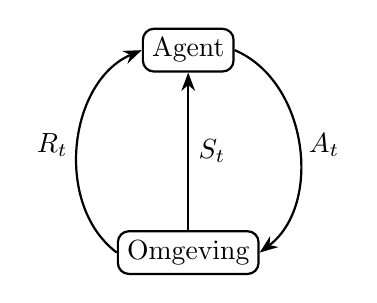
\begin{tikzpicture}[auto, thick, node distance=2cm, >=Stealth]
        % Nodes
        \node[draw, rectangle, rounded corners] (agent) {Agent};
        \node[draw, rectangle, rounded corners, below=of agent] (environment) {Omgeving};

        % Actie-pijl
        \draw[->] (agent.east) to[bend left=60] node[midway, right] {$A_t$} (environment.east);

        % Toestand-pijl
        \draw[->] (environment.north) to node[midway, right] {$S_{t}$} (agent.south);

        % Beloning-pijl
        \draw[->] (environment.west) to[bend left=60] node[midway, left] {$R_{t}$} (agent.west);
    \end{tikzpicture}
    \captionof{figure}{RL model tussen agent en omgeving.}
    \label{fig:rl_model}
\end{minipage}

Dit proces vindt plaats door middel van een vallen en opstaan aanpak, waarbij
de agent beloningen ontvangt voor correcte acties en straffen voor incorrecte
acties(negatieve beloningen). Het uiteindelijke doel is het maximaliseren van
de cumulatieve beloning over tijd.

Computerspellen vormen een ideaal testplatform voor RL vanwege de veelzijdige
uitdagingen die ze bieden, zoals dynamische omgevingen, complexe regels en
onvoorspelbare scenario’s. RL heeft bewezen effectief te zijn in spellen met
zowel discrete als continue actie- en toestandruimtes, variërend van
actiespellen zoals Snake tot strategische spellen zoals Schaken. Het toepassen
van RL in gaming vereist een diep begrip van zowel de kenmerken van de spellen
als de algoritmes die worden ingezet.
\section{Doel van het onderzoek}
Het doel van dit onderzoek is om te begrijpen hoe de kenmerken van
verschillende computerspellen de effectiviteit van verschillende reinforcement
learning (RL) algoritmes beïnvloeden bij het verbeteren van spelprestaties. Dit
onderzoek richt zich op het identificeren van de eigenschappen van
verschillende soorten spellen en de kenmerken van RL-algoritmes.

Door verschillende RL-algoritmes toe te passen op een reeks spellen met
verschillende kenmerken, willen we ontdekken welke algoritmes het beste
presteren in welke soorten spellen. Dit kan variëren van strategische spellen
die planning vereisen tot actiespellen die snelle beslissingen vragen.
\section{Onderzoeksvragen}
\subsection*{Hoofdvraag}
Hoe beïnvloeden de specifieke kenmerken van computerspellen de effectiviteit
van verschillende reinforcement learning-algoritmes in het optimaliseren van
spelprestaties?
\subsection*{Deelvragen}
Om beter te begrijpen hoe de kenmerken van computerspellen de prestaties van
verschillende reinforcement learning (RL) algoritmes beïnvloeden, hebben we
drie belangrijke deelvragen opgesteld
\begin{enumerate}

    \item\subsubsection*{Wat zijn de specifieke kenmerken van verschillende soorten computerspellen?}
          Deze vraag richt zich de eigenschappen van
          verschillende soorten computerspellen. Spellen kunnen sterk verschillen in
          hoe ze zijn opgebouwd, hoe snel spelers beslissingen moeten nemen en hoe
          complex de spelregels zijn. Door deze kenmerken te onderzoeken, kunnen
          we inzicht krijgen in welke aspecten van een spel een uitdaging vormen voor RL-algoritmes.

    \item\subsubsection*{Welke reinforcement learning-algoritmes zijn beschikbaar en wat zijn hun
              kenmerken?}
          Hier willen we kijken naar de verschillende soorten RL-algoritmes die beschikbaar
          zijn en wat hen uniek maakt. Sommige algoritmes zijn beter in het leren van eenvoudige
          taken, terwijl andere juist goed zijn in het omgaan met complexe situaties.

    \item\subsubsection*{Hoe beïnvloeden de spelkenmerken de prestatie van reinforcement learning-algoritmes?}

          Deze vraag gaat in op het belangrijkste deel van het onderzoek: het verband
          tussen de kenmerken van een spel en hoe goed een RL-algoritme presteert. We
          willen weten hoe bepaalde eigenschappen van een spel, zoals de noodzaak voor
          snelle beslissingen of lange-termijnplanning, invloed hebben op de
          effectiviteit van een algoritme. Door de prestaties van verschillende
          algoritmes in verschillende spellen te vergelijken, kunnen we ontdekken welke
          het beste werken voor bepaalde soorten spellen en waarom dat zo is.

\end{enumerate}
\section{Hypothese}
We verwachten dat:
\begin{enumerate}
    \item Deep Q-Network het beste zal presteren in Snake omdat het algoritme snel kan
          leren in omgevingen met beperkte ruimte en snel veranderende situaties, waar
          directe beloningen een grote rol spelen.

    \item Proximal Policy Optimization zal beter presteren in Mario Super Bros, omdat dit
          algoritme geschikt is voor dynamische omgevingen en situaties waar zowel
          snelheid en planning belangrijk zijn.

    \item AlphaZero zal beter zijn in Schaken, vanwege het planning en
          lange-termijnstrategie die nodig zijn.

\end{enumerate}

\section{Relevantie van het Onderzoek}
Dit onderzoek laat effectiviteit van reinforcement learning algoritmes in
verschillende omgevingen laat zien, wat bijdraagt aan het beter gebruik van
KI-systemen. Deze kennis kan niet alleen worden toegepast binnen de
game-industrie, maar ook in andere sectoren zoals de gezondheidszorg,
zelfrijdende auto's en robotica.

\chapter{Theoretisch Kader}

Reinforcement Learning (RL) opereert binnen het kader van Markov Decision
Processes (MDP's), die een wiskundige basis bieden voor het modelleren van
sequentiële beslissingsproblemen. Dit hoofdstuk bespreekt de fundamentele
concepten en wiskundige formuleringen die ten grondslag liggen aan RL,
gestructureerd rond vier kernonderdelen: de basiselementen van MDP's, de
Markov-eigenschap en overgangsdynamiek, beleid en waarde-functies, en de
Bellman-vergelijkingen.

\section{Fundamentele Elementen van MDP's}

\subsection{Toestandsruimte}
Laat (\(\mathcal{X}\)) de toestandsruimte zijn, waarbij elke toestand (\(x \in
\mathcal{X}\)) de huidige situatie of staat is van de omgeving waarin de agent
opereert. Op de aanvangsstap (\(t = 0\)) begint de agent in een initiële
toestand (\(x_0\)). Naarmate het proces vordert, bevindt de agent zich in
nieuwe toestanden gebaseerd op zijn acties.

\subsection{Actieruimte}
Laat (\(\mathcal{A}\)) de actieruimte zijn, waarbij elke actie (\(a \in
\mathcal{A}\)) een mogelijke beslissing van de agent vertegenwoordigt. De
interactie tussen de agent en de omgeving verloopt in discrete tijdstappen (\(t
= 0, 1, 2, \ldots, T\)), waarbij de horizon (\(T\)) eindig of oneindig kan
zijn.

\subsection{Beloningsfunctie}
De beloningsfunctie (\(r: \mathcal{X} \times \mathcal{A} \to \mathbb{R}\))
koppelt toestand-actieparen aan beloningen, waarbij (\(r(x,a)\)) de directe
beloning vertegenwoordigt die wordt ontvangen na het uitvoeren van actie
(\(a\)) in toestand (\(x\)).

\section{Markov-eigenschap en Overgangsdynamiek}

\subsection{De Markov-eigenschap}
Het onderscheidende kenmerk van MDP's is de Markov-eigenschap, die stelt dat de
toekomstige toestand alleen afhankelijk is van de huidige toestand en actie,
onafhankelijk van de geschiedenis:
\[
    p(x_{t+1}|x_t,a_t,x_{t-1},a_{t-1},\ldots,x_0,a_0) = p(x_{t+1}|x_t,a_t)
\]
Voorbeeld van het Markov-eigenschap:
\begin{itemize}
    \item \textbf{Snake}: De toekomstige toestand (positie van de slang en voedsel) is volledig bepaald door de huidige toestand (huidige positie en locatie van het voedsel) en de actie (richting van beweging) zonder afhankelijk te zijn van de geschiedenis van eerdere bewegingen.
\end{itemize}

Voorbeeld van geen Markov-eigenschap:
\begin{itemize}
    \item \textbf{Poker}: De beslissingen in poker zijn afhankelijk van niet alleen de huidige hand, maar ook van de geschiedenis van inzetten en het gedrag van andere spelers in vorige rondes.
\end{itemize}

\subsection{Overgangswaarschijnlijkheidsfunctie}
Voor eindige toestands- en actieruimten (\(|\mathcal{X}|, |\mathcal{A}| <
\infty\)) worden de overgangsdynamieken beschreven door een
waarschijnlijkheidsfunctie (\(p: \mathcal{X} \times \mathcal{A} \times
\mathcal{X} \to [0,1]\)), waarbij (\(p(x'|x,a)\)) de waarschijnlijkheid
vertegenwoordigt om over te gaan naar toestand (\(x'\)) gegeven de huidige
toestand (\(x\)) en actie (\(a\)).

\section{Beleid en Verwachte Waarden}

\subsection{Beleid}
In RL is een beleid de strategie die een agent volgt om beslissingen te nemen.
Het bepaalt welke actie een agent moet uitvoeren, gegeven de huidige toestand
van de omgeving. Een beleid in reinforcement learning kan op twee manieren
worden gedefinieerd:

\begin{itemize}
    \item \textbf{Deterministisch Beleid:} \\
          \(\pi: \mathcal{X} \to \mathcal{A}\), waarbij \(a_t = \pi(x_t)\) \\
          Voor elke toestand \(x_t\) schrijft het beleid exact één actie \(a_t\) voor.

    \item \textbf{Stochastisch Beleid:} \\
          \(\pi: \mathcal{X} \times \mathcal{A} \to [0,1]\), waarbij \(\pi(a|x)\) de waarschijnlijkheid geeft van het kiezen van actie \(a\) in toestand \(x\) \\
          Voor een gegeven toestand \(x\) definieert het beleid een waarschijnlijkheidsverdeling over mogelijke acties.
\end{itemize}

\subsection{Verwachte Waarden}
De verwachtingswaarde \(\mathbb{E}[X]\) (Expected value), of het gemiddelde,
van een willekeurige variabele \(X\) is een manier om het gemiddelde resultaat
te berekenen dat je zou verwachten als je een groot aantal experimenten
uitvoert. Bijvoorbeeld, als \(X\) een dobbelsteenworp vertegenwoordigt, dan is
\(\mathbb{E}[X]\) het gemiddelde van de uitkomsten 1, 2, 3, 4, 5, en 6, wat
gelijk is aan 3,5. De conditionele verwachting (\(\mathbb{E}[X|Y]\)) geeft de
verwachte waarde van (\(X\)) gegeven (\(Y\)).

\subsection{Kortingsfactor}
De kortingsfactor (\(\gamma \in [0,1]\)) bepaalt het gewicht bepaalt van
toekomstige beloningen ten opzichte van onmiddellijke beloningen, waarbij:

\begin{itemize}
    \item (\(\gamma = 0\)) alleen directe beloningen hebben invloed
    \item (\(\gamma = 1\)) alle toekomstige beloningen zijn even invloedrijk
    \item (\(0 < \gamma < 1\)) een korting toepast op toekomstige beloningen
\end{itemize}

\section{Waarde-functies en Bellman-vergelijkingen}
De toestandswaarde-functie geeft aan hoe goed een bepaalde toestand is, terwijl
de Q-functie aangeeft hoe goed een actie in een bepaalde toestand is.
\subsection{Toestandswaarde-functie}
De toestandswaarde-functie (\(V^\pi: \mathcal{X} \to \mathbb{R}\)) onder beleid
(\(\pi\)) wordt gedefinieerd als:
\[
    V^\pi(x) = \mathbb{E}_\pi\left[\sum_{t=0}^\infty \gamma^t r_t \mid x_0 = x\right]
\]
Deze functie geeft de verwachte waarde van de totale beloning die een agent zal
ontvangen vanaf de toestand \(x\).
\subsection{Q-functie}
De Q-functie (\(Q^\pi: \mathcal{X} \times \mathcal{A} \to \mathbb{R}\)) onder
beleid (\(\pi\)) wordt gedefinieerd als:
\[
    Q^\pi(x,a) = \mathbb{E}_\pi\left[\sum_{t=0}^\infty \gamma^t r_t \mid x_0 = x, a_0 = a\right]
\]
Deze functie geeft de verwachte waarde van de totale beloning die een agent zal
ontvangen vanaf de toestand \(x\) en na het nemen van actie \(a\).

\subsection{Bellman-vergelijkingen}
De Bellman-vergelijkingen drukken de recursieve relatie uit tussen waarden van
opeenvolgende toestanden:
\begin{itemize}
    \item Toestandswaarde Bellman-vergelijking:
          \[
              V^\pi(x) = \mathbb{E}_{a \sim \pi(\cdot|x), x' \sim p(\cdot|x,a)}[r(x,a) + \gamma V^\pi(x')]
          \]
    \item Actiewaarde Bellman-vergelijking:
          \[
              Q^\pi(x,a) = \mathbb{E}_{x' \sim p(\cdot|x,a), a' \sim \pi(\cdot|x')}[r(x,a) + \gamma Q^\pi(x',a')]
          \]
\end{itemize}
De relatie tussen (\(V^\pi\)) en (\(Q^\pi\)) wordt gegeven door:
\[
    V^\pi(x) = \mathbb{E}_{a \sim \pi(\cdot|x)}[Q^\pi(x,a)]
\]

\section{Leerparadigma's}
\subsection{Model-Based vs Model-Free Learning}
\subsubsection{Model-Based Learning}
Bij model-based learning construeert de agent expliciet een model (\(\hat{p}\))
van de overgangsdynamiek en beloningsfunctie van de omgeving (\(\hat{r}\)). Het
geleerde model benadert:

\begin{itemize}
    \item Overgangsfunctie: \(\hat{p}(x'|x,a) \approx p(x'|x,a)\)
    \item Beloningsfunctie: \(\hat{r}(x,a) \approx r(x,a)\)
\end{itemize}

De agent kan dit model gebruiken voor:

\begin{itemize}
    \item \textit{Planning}: Het simuleren van trajecten zonder interactie met de omgeving.
    \item \textit{Counterfactual reasoning}: Het evalueren van acties die niet daadwerkelijk zijn uitgevoerd.
\end{itemize}

\subsubsection{Model-Free Learning}
Model-free methoden leren waardefuncties of beleidsregels direct uit ervaring,
zonder een expliciet model te construeren. Deze methoden werken door:

\begin{itemize}
    \item Directe updates van waarde-schattingen.
    \item Beleidsverbetering op basis van gesamplede trajecten.
    \item Geen expliciete representatie van overgangsdynamiek.
\end{itemize}

\subsection{On-Policy vs Off-Policy Learning}
\subsubsection{On-Policy Learning}
On-policy methoden leren over het beleid dat momenteel wordt uitgevoerd. De
update van de waardefunctie volgt:
\[
    \text{Target} = r + \gamma \mathbb{E}_{a' \sim \pi(\cdot|x')}[Q(x',a')]
\]
waarbij \(\pi\) zowel:

\begin{itemize}
    \item Het gedragsbeleid (dat ervaringen genereert) als
    \item Het doelbeleid (dat wordt geleerd) is.
\end{itemize}

\subsubsection{Off-Policy Learning}
Off-policy methoden leren over één beleid (\(\pi\)) terwijl een ander beleid
(\(\mu\)) wordt gevolgd. Dit omvat:

\begin{itemize}
    \item \textit{Gedragsbeleid} (\(\mu\)): Gebruikt voor exploratie.
    \item \textit{Doelbeleid} (\(\pi\)): Het beleid dat wordt geleerd.
\end{itemize}

De importance sampling ratio (\(\rho\)) corrigeert voor het verschil tussen de
]beleidsregels:
\[
    \rho_t = \frac{\pi(a_t|x_t)}{\mu(a_t|x_t)}
\]
Dit maakt het mogelijk om te leren over optimaal gedrag terwijl een exploratief
beleid wordt gevolgd.


\chapter*{Theoretisch Kader}

\section*{Definitie}
Een actie is de beslissing die een agent neemt bij elke stap in een
besluitvormingsproces. Acties worden aangeduid met \( a \) en worden gekozen
uit een reeks mogelijke acties \( \mathcal{A} \). Elke door de agent genomen
actie beïnvloedt de interactie met de omgeving, wat leidt tot een verandering
in de toestand en een daaruit voortvloeiende beloning.

Een toestand \( x \) vertegenwoordigt de huidige situatie of staat van de
omgeving waarin de agent opereert. Dit wordt aangeduid met \( x \) en maakt
deel uit van de toestandsruimte \( \mathcal{X} \). Bij de aanvangsstap \( t = 0
\), begint de agent in een initiële toestand \( x_0 \) die willekeurig wordt
bepaald door een verdeling \( p \). Naarmate het proces vordert, bevindt de
agent zich in nieuwe toestanden gebaseerd op zijn acties.

Een beloning \( r \) is een feedbackwaarde die wordt ontvangen nadat de agent
een actie heeft uitgevoerd in een bepaalde toestand. Deze beloning wordt
bepaald door de beloningsfunctie \( r(x, a) \). De beloningsmatrix \( R \)
bevat de onmiddellijke beloningen voor elke combinatie van toestand en actie.

Een overgang beschrijft de verandering van de huidige toestand naar de volgende
toestand als gevolg van een actie die door de agent wordt genomen. De
waarschijnlijkheid van overgang wordt bepaald door de
overgangswaarschijnlijkheidsfunctie \( p(x'|x, a) \), die afhangt van de
huidige toestand \( x \), de genomen actie \( a \) en leidt tot een nieuwe
toestand \( x' \). De overgangswaarschijnlijkheidsmatrix \( P \) bevat de
waarschijnlijkheden van het overgaan van de ene toestand naar de volgende
toestand, gegeven een bepaalde actie.

\subsection*{Markov-eigenschap}

MDP werkt onder de Markov-aanname, wat betekent dat de volgende toestand en
beloning alleen afhangen van het huidige toestand-actiepaar en niet van enige
eerdere geschiedenis. Deze eigenschap vereenvoudigt het besluitvormingsmodel
door zich alleen te concentreren op de huidige situatie.

Voorbeeld van een MDP:
\begin{itemize}
    \item \textbf{Snake}: De toekomstige toestand (positie van de slang en voedsel) is volledig bepaald door de huidige toestand (huidige positie en locatie van het voedsel) en de actie (richting van beweging) zonder afhankelijk te zijn van de geschiedenis van eerdere bewegingen.
\end{itemize}

Voorbeeld van geen MDP:
\begin{itemize}
    \item \textbf{Poker}: De beslissingen in poker zijn afhankelijk van niet alleen de huidige hand, maar ook van de geschiedenis van inzetten en het gedrag van andere spelers in vorige rondes.
\end{itemize}

Voorbeeld van een twijfelgeval:
\begin{itemize}
    \item \textbf{Schaak}: Elke positie op het bord (toestand) en mogelijke zetten (acties) bepalen de volgende positie, maar strategieën kunnen afhankelijk zijn van eerdere zetten.
\end{itemize}

In een MDP gaat een agent verder in tijdstappen \(t = 0, 1, 2, \ldots, T\) waar
de horizon \(T\) zowel eindig als oneindig kan zijn. Hierin is \(T\) oneindig
tenzij anders aangegeven.

\subsection*{Overgangswaarschijnlijkheidsmatrix}

Wanneer de set van alle toestanden \(\mathcal{X}\) en de set van alle acties
\(\mathcal{A}\) eindig zijn, d.w.z. \(|\mathcal{X}|, |\mathcal{A}| < \infty\),
kan de overgangswaarschijnlijkheidsfunctie \(p(x'|x,a)\) worden weergegeven als
een overgangsmatrix.

De grootte van de overgangswaarschijnlijkheidsmatrix is \(|\mathcal{X}| \times
|\mathcal{X}| \times |\mathcal{A}|\). Dit is een driedimensionale matrix. De
dimensies zijn als volgt:
\begin{itemize}
    \item De huidige toestand \(x\).
    \item De genomen actie \(a\).
    \item De volgende toestand \(x'\).
\end{itemize}

\subsection*{Beleid}

In RL is een beleid de strategie die een agent volgt om beslissingen te nemen.
Het bepaalt welke actie een agent moet uitvoeren, gegeven de huidige toestand
van de omgeving. Er zijn twee hoofdtypen beleid:

\begin{itemize}
    \item \textbf{Deterministisch Beleid}:
          \begin{itemize}
              \item \textbf{Formule:} \(a_t = \pi(s_t)\)
              \item \textbf{Beschrijving:} Voor elke toestand \(s_t\) kiest het beleid altijd dezelfde actie \(a_t\). Het resultaat is volledig voorspelbaar zolang de toestand bekend is.
          \end{itemize}

    \item \textbf{Stochastisch Beleid}:
          \begin{itemize}
              \item \textbf{Formule:} \(a_t \sim \pi(\cdot|s_t)\)
              \item \textbf{Beschrijving:} Voor een gegeven toestand \(s_t\) kiest het beleid een actie \(a_t\) volgens een waarschijnlijkheidsverdeling. Dit betekent dat de actie die wordt gekozen afhankelijk is van kans, wat leidt tot variabiliteit in het gedrag van de agent.
          \end{itemize}
\end{itemize}

\subsection*{Verwachtingswaarde}

De verwachtingswaarde \(\mathbb{E}[X]\) (Expected value), of het gemiddelde,
van een willekeurige variabele \(X\) is een manier om het gemiddelde resultaat
te berekenen dat je zou verwachten als je een groot aantal experimenten
uitvoert. Bijvoorbeeld, als \(X\) een dobbelsteenworp vertegenwoordigt, dan is
\(\mathbb{E}[X]\) het gemiddelde van de uitkomsten 1, 2, 3, 4, 5, en 6, wat
gelijk is aan 3,5.

\textbf{Geconditioneerde verwachtingswaarde} \(\mathbb{E}[a|b]\): het gemiddelde van \(a\) berekenen, gegeven de voorwaarde \(b\).

\subsection*{Kortingsfactor}

De kortingsfactor \(\gamma\) is een getal tussen 0 en 1 dat het gewicht bepaalt
van toekomstige beloningen ten opzichte van onmiddellijke beloningen. Bij een
lage kortingsfactor hebben toekomstige beloningen weinig invloed. Bij een
kortingsfactor van 1 hebben alle beloningen evenveel invloed.

\subsection*{Waardefunctie}

De waardefunctie \(V(x)\) geeft de verwachte waarde van de totale beloning die
een agent zal ontvangen vanaf de toestand \(x\) als hij het beleid \(\pi\)
volgt.

\[
    V(x) := \mathbb{E}_{\pi}\left[\sum_{t=0}^{\infty} \gamma^t r_t \mid x_0 = x\right]
\]

Hierin is \(\sum_{t=0}^{\infty} \gamma^t r_t\) de som van alle beloningen
waarbij elke beloning wordt vermenigvuldigd met \(\gamma^t\) als de
kortingsfactor (\(\gamma \in [0,1]\)). Dan wordt elke beloning met een groter
tijdstapje (verder in de toekomst) kleiner en heeft dus minder invloed op de
verwachte waarde.

\subsection*{Q-functie}

De Q-functie \(Q(x,a)\) geeft de verwachte waarde van de totale beloning die
een agent zal ontvangen vanaf de toestand \(x\) en na het nemen van actie
\(a\), als hij daarna het beleid \(\pi\) volgt.

\[
    Q(x,a) := \mathbb{E}_{\pi}\left[\sum_{t=0}^{\infty} \gamma^t r_t \mid x_0 = x, a_0 = a\right]
\]

\noindent waarin \(a_0 = a\) betekent dat de eerste actie \(a\) is.

De waardefunctie geeft aan hoe goed een bepaalde toestand is, terwijl de
Q-functie aangeeft hoe goed een actie in een bepaalde toestand is.

Waarde functie en Q-functie zijn gerelateerd aan elkaar op deze manier:

\[
    V(x) = \mathbb{E}_{a \sim \pi(\cdot|x)}[Q(x,a)]
\]

\subsection*{Bellman vergelijking}

De Q-functie en de waardefunctie in RL moeten voldoen aan
consistentievoorwaarden, bekend als de Bellman-vergelijkingen. Voor een gegeven
beleid \(\pi\), kunnen de waardefunctie \(V(x)\) en de Q-functie \(Q(x,a)\) als
volgt worden gedefinieerd:

\[
    V(x) = \mathbb{E}_{a \sim \pi(\cdot|x), x' \sim p(\cdot|x,a)}[r(x,a) + \gamma V(x')]
\]

\[
    Q(x,a) = \mathbb{E}_{x' \sim p(\cdot|x,a), a' \sim \pi(\cdot|x')}[r(x,a) + \gamma Q(x',a')]
\]

\noindent waarin:
\begin{itemize}
    \item \(a \sim \pi(\cdot|x)\) betekent dat actie \(a\) de actie is volgens beleid \(\pi\) in toestand \(x\).
    \item \(x' \sim p(\cdot|x,a)\) betekent dat toestand \(x'\) volgt uit toestand \(x\) en actie \(a\) volgens de overgangswaarschijnlijkheidsfunctie \(p\).
    \item \(a' \sim \pi(\cdot|x')\) betekent dat de volgende actie \(a'\) de actie is volgens beleid \(\pi\) in de nieuwe toestand \(x'\).
    \item \(r(x,a)\) is de beloning van actie \(a\) in toestand \(x\).
\end{itemize}

\subsection*{Evaluatie en Controle}

Er zijn twee problemen in RL:
\begin{itemize}
    \item \textbf{Evaluatie:} Het eerste probleem in RL is evaluatie. Het doel is om te berekenen hoe goed een bepaald beleid \(\pi\) presteert. Dit wordt gedaan door te kijken naar de waarde functie \(V(x)\) of de Q-functie \(Q(x,a)\).

          Waarom is evaluatie een probleem?
          \begin{itemize}
              \item \textbf{Complexiteit van de omgeving:} In een dynamische omgeving kan het moeilijk zijn om te voorspellen welke beloningen een agent zal ontvangen vanuit een bepaalde toestand, vooral als de omgeving verandert zonder dat de agent verandert.
              \item \textbf{Variabiliteit van beloningen:} Beloningen kunnen stochastisch zijn, wat betekent dat dezelfde actie in dezelfde toestand verschillende uitkomsten kan hebben.
              \item \textbf{Lange termijn effecten:} Het effect van een bepaalde actie wordt pas later zichtbaar.
          \end{itemize}

          Het evaluatieprobleem wordt meestal beschouwd als een subroutine van het tweede
          probleem: controle.

    \item \textbf{Controle:} Bij controle is het doel om het beleid \(\pi\) te vinden dat de waarde functie maximaliseert over de initiële toestanden \(x \sim \rho\).

          \[
              \max_{\pi} \mathbb{E}_{x \sim \rho}[V(x)]
          \]

          \noindent waarin \(x \sim \rho\) betekent dat de toestand \(x\) van de agent komt uit een vooraf gedefinieerde verzameling toestanden, waarbij elke toestand een bepaalde kans heeft om gekozen te worden.

          Waarom is controle een probleem?
          \begin{itemize}
              \item \textbf{Exploratie vs. exploitatie:} De agent moet een balans vinden tussen het verkennen van nieuwe acties om betere beloningen te ontdekken (exploratie) en het uitbuiten van bekende acties die momenteel de hoogste beloning bieden (exploitatie).
              \item \textbf{Dimensionale complexiteit:} In veel RL-toepassingen zijn er een groot aantal toestanden en acties, wat het zoeken naar het optimale beleid computationeel duur maakt.
          \end{itemize}

          Het optimale beleid \(\pi^*\) is het beleid dat de verwachte cumulatieve
          beloning over tijd maximaliseert.

          \[
              Q^*(x,a) = \mathbb{E}_{x' \sim p(\cdot|x,a)}\left[r(x,a) + \gamma \max_{a'} Q^*(x',a')\right]
          \]
\end{itemize}

\chapter{Kenmerken van specifieke Algoritmes}

\section{Q-Learning}
Q-learning, geïntroduceerd door Chris Watkins in 1989, is een van de
belangrijkste vooruitgangen binnen reinforcement learning. Dit model-vrije,
off-policy algoritme is een van de meest gebruikte algoritmen binnen
reinforcement learning vanwege zijn eenvoud en effectiviteit.
\subsection{Proces}
Het proces van het Q-learning-algoritme, zoals weergegeven in
\textbf{Algoritme~\ref{alg:Q-learning}} en de flowchart in
\textbf{Figuur~\ref{fig:ql_flowchart}}, begint met het opstellen van een
Q-tabel. Deze tabel bevat de Q-waarden voor alle combinaties van toestanden en
acties. Aan het begin zijn alle waarden ingesteld op nul.

Vervolgens start het spel, waarbij de agent de volgende actie bepaalt. Hierbij
heeft de agent twee mogelijkheden:
\begin{itemize}
    \item Exploratie: De agent voert een willekeurige actie uit om nieuwe informatie te
          verkennen.
    \item Exploitatie: De agent selecteert een actie op basis van de bestaande Q-tabel,
          waarbij de actie met de hoogste Q-waarde in de huidige toestand wordt gekozen.
\end{itemize}

De keuze tussen exploratie en exploitatie wordt bepaald door de parameter
$\epsilon$. De kans dat de agent een willekeurige actie uitvoert (exploratie)
is gelijk aan $\epsilon$. Aan het begin van de training is $\epsilon$ gelijk
aan 1, en deze waarde neemt exponentieel af naarmate de training vordert. Tegen
het einde van de training is $\epsilon$ vrijwel 0.

Nadat een actie is uitgevoerd, ontvangt de agent een beloning. Op basis van
deze beloning wordt de Q-waarde voor de combinatie van de uitgevoerde actie en
de huidige toestand bijgewerkt in de Q-tabel. Dit proces wordt herhaald totdat
de training is voltooid.
\subsection{Convergentie en Optimaliteit}
\subsection{Voordelen en Beperkingen}
\subsection{Toepassingen van Q-learning}

\begin{algorithm}
    \caption{Q-Learning Algoritme}\label{alg:Q-learning}
    \begin{algorithmic}
        \State \textbf{Initialisatie:} Stel $Q(s, a)$ willekeurig in voor alle toestanden $s$ en acties $a$
        \For{elke episode}
        \State Initialiseer begin-toestand $s$
        \While{$s$ is niet een terminale toestand}
        \State Kies actie $a$ in toestand $s$ op basis van een beleid $\pi$
        \State Voer actie $a$ uit, observeer beloning $r$ en de volgende toestand $s'$
        \State Update de Q-waarde:
        \[
            Q(s, a) \gets Q(s, a) + \alpha \left[ r + \gamma \max_{a'} Q(s', a') - Q(s, a) \right]
        \]
        \State $s \gets s'$
        \EndWhile
        \EndFor
    \end{algorithmic}
\end{algorithm}

\begin{figure}
    \centering
    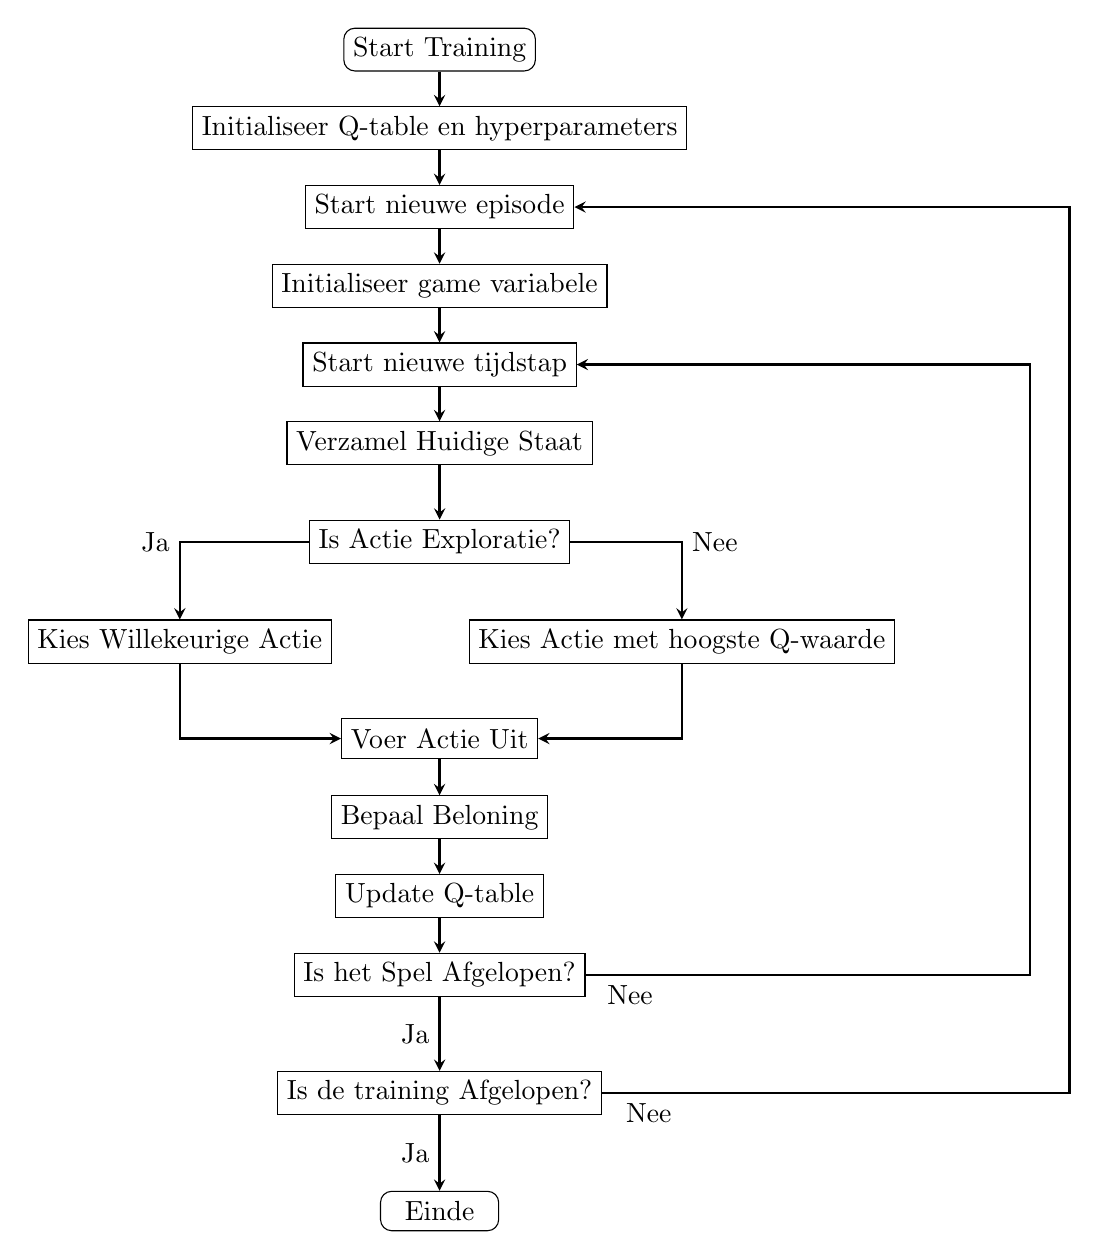
\begin{tikzpicture}[node distance=1cm, auto, >=latex']
        % Definieer stijlen voor verschillende soorten knooppunten
        \tikzstyle{startstop} = [rectangle, rounded corners, minimum width=1.5cm, minimum height=0.5cm,text centered, draw=black, fill=red!0]
        \tikzstyle{process} = [rectangle, minimum width=1.5cm, minimum height=0.5cm, text centered, draw=black, fill=orange!0]
        \tikzstyle{decision} = [rectangle, minimum width=1.5cm, minimum height=0.5cm, text centered, draw=black, fill=green!0]
        \tikzstyle{arrow} = [thick,->,>=stealth]

        % Knopen plaatsen
        \node (start) [startstop] {Start Training};
        \node (trainingInit) [process, below of=start] {Initialiseer Q-table en hyperparameters};
        \node (startEpisode) [process, below of=trainingInit] {Start nieuwe episode};
        \node (episodeInit) [process, below of=startEpisode] {Initialiseer game variabele};
        \node (startTimestep) [process, below of=episodeInit] {Start nieuwe tijdstap};
        \node (getstate) [process, below of=startTimestep] {Verzamel Huidige Staat};
        \node (decideexplore) [decision, below of=getstate, yshift=-0.25cm] {Is Actie Exploratie?};
        \node (explore) [process, below left=of decideexplore, xshift=1cm] {Kies Willekeurige Actie};
        \node (exploit) [process, below right=of decideexplore, xshift=-2cm] {Kies Actie met hoogste Q-waarde};
        \node (executeaction) [process, below of=decideexplore, yshift=-1.5cm] {Voer Actie Uit};
        \node (determinereward) [process, below of=executeaction] {Bepaal Beloning};
        \node (updateq) [process, below of=determinereward] {Update Q-table};
        \node (checkgameover) [decision, below of=updateq] {Is het Spel Afgelopen?};
        \node (checktrainingover) [decision, below of=checkgameover, yshift=-0.5cm] {Is de training Afgelopen?};
        \node (stop) [startstop, below of=checktrainingover, yshift=-0.5cm] {Einde};

        % Pijlen tekenen
        \draw [arrow] (start) -- (trainingInit);
        \draw [arrow] (trainingInit) -- (startEpisode);
        \draw [arrow] (startEpisode) -- (episodeInit);
        \draw [arrow] (episodeInit) -- (startTimestep);
        \draw [arrow] (startTimestep) -- (getstate);
        \draw [arrow] (getstate) -- (decideexplore);
        \draw [arrow] (decideexplore) -| node[anchor=east] {Ja} (explore);
        \draw [arrow] (decideexplore) -| node[anchor=west] {Nee} (exploit);
        \draw [arrow] (explore) |- (executeaction);
        \draw [arrow] (exploit) |- (executeaction);
        \draw [arrow] (executeaction) -- (determinereward);
        \draw [arrow] (determinereward) -- (updateq);
        \draw [arrow] (updateq) -- (checkgameover);
        \draw [arrow] (checkgameover) -- node[anchor=east] {Ja} (checktrainingover);
        \draw [arrow] (checkgameover) -| node[pos=0.05, anchor=north, align=center] {Nee} (7.5,-4) -- (startTimestep);
        \draw [arrow] (checktrainingover) -- node[anchor=east] {Ja} (stop);
        \draw [arrow] (checktrainingover) -| node[pos=0.05, anchor=north, align=center] {Nee} (8,-2) -- (startEpisode);
    \end{tikzpicture}
    \caption{Flowchart van het Q-Learning Algoritme}\label{fig:ql_flowchart}
\end{figure}

\newpage

\section{Deep Q-Network}

\section{AplhaZero}

\chapter{Kenmerken van specifieke Computerspellen}
Er zijn talloze computerspellen met diverse en uitdagende omgevingen voor de
toepassing van reinforcement learning (RL)-algoritmes. Spellen onderling kunnen
erg van elkaar variëren onder andere in structuur, dynamiek, complexiteit, en
tijdsduur. Al deze aspecten kunnen dergelijke invloed hebben op de
effectiviteit van RL-algoritmes. Elk type spel stelt specifieke eisen aan een
RL-algoritme, afhankelijk van aspecten zoals de omvang van de toestandsruimte,
de regels en beperkingen, en de vereiste strategische vaardigheden.

In dit hoofdstuk worden de specifieke kenmerken van vier computerspellen met
elkaar vergeleken: een \textit{auto-racespel} waar de agent het
autobesturingssysteem is, \textit{Snake} waar de agent de slang is,
\textit{Schaken} waar de agent de schaker is en \textit{Super Mario Bros} waar
de agent Mario is. Een overzicht van alle speleigenschappen is te zien in Tabel
??.

\section{Indeling en Strategische Diepgang van Spellen} Spellen kunnen worden ingedeeld op basis van hun genre en de mate van
strategische diepgang die nodig is om succesvol te zijn. Actie- en
platformspellen, zoals \textit{Super Mario Bros}, hebben een gemiddelde
strategische diepgang. Het doel is obstakels te overwinnen, vijanden te
ontwijken of verslaan en tegelijkertijd gouden munten te verzamelen. Dit soort
spellen vereist doorgaans korte termijn optimalisatie en directe reacties.

Strategiespellen, zoals \textit{Schaken}, vragen daarentegen om diepgaande
planning en vooruitdenken. Hier moet een speler of agent een reeks mogelijke
toekomstige toestanden analyseren en anticiperen op de acties van een
tegenstander. De strategische diepgang maakt leren complex, omdat beloningen
vaak cumulatief en pas aan het einde van het spel duidelijk worden. Dergelijke
spellen vereisen geavanceerde reinforcement learning (RL)-algoritmes die
langetermijnplanning ondersteunen.

Puzzel-/actiespellen, zoals \textit{Snake}, zijn minder afhankelijk van
strategie. Hier draait het om patroonherkenning en korte termijn optimalisatie,
waarbij eenvoudige RL-algoritmes voldoende zijn om succesvol te leren. Het doel
is bijvoorbeeld appels te verzamelen zonder jezelf te raken, waarbij de
beloningsstructuur rechtlijnig is.

Simulatie- en racegames, zoals een racespel met een zelfrijdende auto, richten
zich op efficiënt en veilig navigeren over een parcours. Hier ligt de nadruk op
het optimaliseren van gedrag in een gesimuleerde omgeving, vaak zonder de
noodzaak van complexe planningsstrategieën.

Deze variatie in genres en strategische eisen bepaalt welk type RL-algoritme
het meest geschikt is voor een spel. Complexere spellen met hogere strategische
diepgang vereisen geavanceerdere algoritmes, terwijl eenvoudigere spellen vaak
volstaan met directe responsmechanismen.

\section{Indeling van Spellen}
\textit{Super Mario Bros} valt binnen het genre van actie- en platformspellen. Het doel van het spel is over hindernissen springen en vijanden te ontwijken en verslaan en tegelijkertijd gouden munten te verzamelen. \textit{Schaken} daarentegen is een strategiespel, dat volledig turn-based is en gericht op denkvermogen, vooruitdenken en strategische planning. \textit{Snake} wordt vaak als een puzzel-/actiespel beschouwd, waarbij het doel is een appel te eten terwijl je niet jezelf raakt; hier is patroonherkenning belangrijk. Een zelfrijdende auto in een racespel valt binnen het genre van simulatie en racegames. Het draait om het efficiënt en veilig navigeren over een parcours. Dit wordt vaak gebruikt bij offline racespellen waar je tegen de computer speelt.

\section{Strategische Diepgang}
De mate van strategische diepgang in een spel is een van de belangrijkste
factoren die bepalen welk type RL-algoritme geschikt is. Strategie verwijst
naar het vermogen om vooruit te denken en acties te plannen die op lange
termijn voordelig zijn. Dit varieert sterk tussen spellen.

Strategische spellen, zoals \textit{Schaken}, vereisen vereisen dat een agent
ver vooruit denkt en een reeks mogelijke toekomstige toestanden analyseert.
Hier is langetermijnplanning essentieel. De agent moet niet alleen rekening
houden met de huidige toestand, maar ook anticiperen op de mogelijke acties van
een tegenstander en de daaropvolgende uitkomsten. Bij strategische spellen is
het leren complex, omdat beloningen vaak cumulatief en pas aan het einde van
het spel duidelijk worden.

Aan de andere kant zijn er spellen zoals \textit{Snake}, waarin strategie een
veel minder belangrijke rol speelt. In deze spellen zijn acties vaak gebaseerd
op eenvoudige regels en is de beste keuze meestal direct duidelijk. Het succes
van een speler hangt hier voornamelijk af van korte termijn optimalisatie.
Dergelijke spellen vereisen relatief eenvoudige RL-algoritmes, die zijn
ontworpen om direct te reageren op beloningen of straffen zonder complexe
planningsstrategieën. De eenvoudige structuur en beloningsmechanismen maken het
leerproces rechtlijnig en efficiënt.

\section{Beslissingsdynamiek en Tijdgevoeligheid}
De snelheid waarmee de omgeving van een spel verandert, bepaalt in grote mate
hoe moeilijk het is voor een RL-agent om effectief te leren en te reageren.

De beslissingsdynamiek verschilt sterk tussen de spellen. \textit{Super Mario
    Bros} vereist snelle real-time beslissingen. De agent moet op het juiste moment
springen of een vijand ontwijken, en timing is hierbij cruciaal. Bij
\textit{Schaken} is er juist geen tijdsdruk; de agent kan lang “nadenken” over
elke zet. \textit{Snake} zit er tussenin: hoewel het spel niet zo snel is als
\textit{Mario}, zit er wel een kleine tijdsdruk achter, maar dit is meestal
verwaarloosbaar. Timing en patroonherkenning worden belangrijker naarmate het
spel vordert. Bij een zelfrijdende auto in een racespel ligt de
beslissingsdynamiek real-time. Hier zijn snelheid en precisie van beslissingen
belangrijk, omdat milliseconden het verschil kunnen maken tussen een
succesvolle race en een botsing.

\section{Complexiteit}
De complexiteit van de regels en doelen varieert sterk. \textit{Super Mario
    Bros} heeft relatief eenvoudige regels: de agent moet vijanden vermijden en
verslaan, munten verzamelen, en het einde van het level bereiken. De
complexiteit van de vijanden en het terrein neemt echter toe naarmate de levels
moeilijker worden. \textit{Schaken} heeft relatief eenvoudige basisregels: zes
verschillende stukken met elk unieke bewegingsmogelijkheden. Het doel, het
schaakmat zetten van de tegenstander, vereist echter strategisch inzicht en
planning. Dit maakt \textit{Schaken} bijzonder uitdagend voor een RL-agent
vanwege de enorme toestandsruimte en de langetermijnplanning die nodig is.
\textit{Snake} heeft zeer eenvoudige regels: de agent moet voedsel verzamelen
en mag niet botsen met de muur of zichzelf. De uitdaging ligt in de toenemende
snelheid en lengte van de slang. Een zelfrijdende auto in een racespel heeft
daarentegen te maken met complexe regels die gebaseerd zijn op realistische
fysica. Het doel is simpel: zo snel mogelijk de finish bereiken.

\subsection{Regels en Beperkingen}
De complexiteit en het aantal regels in een spel spelen een cruciale rol in de
uitdaging die een RL-agent tegenkomt.

\subsubsection{Spellen met veel regels en vaste patronen}
Spellen zoals 4-op-een-rij of boter-kaas-en-eieren hebben een voorspelbare
structuur en strikte regels. De mogelijke zetten en uitkomsten zijn beperkt,
wat het spel eenvoudiger maakt om te modelleren. RL-algoritmes kunnen hier
profiteren van waarschijnlijkheidsmodellen en gestructureerde planning. De
voorspelbaarheid van deze spellen vermindert de onzekerheid in het leerproces.
Een RL-agent kan relatief eenvoudig een optimale strategie leren door alle
mogelijke acties te analyseren en te kiezen voor de meest belonende uitkomst.

\subsubsection{Spellen met weinig regels en veel vrijheid}
Spellen zoals GTA of Call of Duty bieden een grote mate van keuzevrijheid. De
speler kan vrij bewegen in een open wereld, interacties aangaan en talloze
acties uitvoeren. Deze spellen hebben een enorme toestandsruimte, die
driedimensionaal en dynamisch is. Dergelijke spellen vereisen een flexibel en
adaptief RL-algoritme. Het is onrealistisch voor een RL-agent om alle mogelijke
acties en toestanden volledig te doorzoeken. Algoritmes zoals Proximal Policy
Optimization (PPO) zijn hier geschikt. PPO gebruikt stochastische
beleidsmodellen en leert door te experimenteren met acties, waarbij het snel
aanpassingen kan maken op basis van feedback.

\section{Dynamiek en Tijdgevoeligheid}
De snelheid waarmee de omgeving van een spel verandert, bepaalt in grote mate
hoe moeilijk het is voor een RL-agent om effectief te leren en te reageren.

\subsection{Turn-based spellen}
Spellen zoals \textit{Schaken} of Monopoly bieden de speler voldoende tijd om
de optimale actie te berekenen. Omdat de omgeving niet continu verandert, kan
een RL-algoritme worden ingezet om een uitgebreide analyse te maken van alle
mogelijke uitkomsten van een actie. Dit type algoritme is bijzonder effectief
in spellen waar de agent kan profiteren van gestructureerde planning en
voorspelbare omgevingen.

\subsection{Realtime spellen}
In spellen zoals \textit{Mario Bros} of Tetris veranderen de omstandigheden
continu. Obstakels bewegen, vijanden verschijnen en de tijdsdruk vereist snelle
besluitvorming. Voor deze spellen zijn algoritmes nodig die snel leren en
direct reageren, met neurale netwerken, waardoor het algoritme in real-time
beslissingen kan nemen op basis van eerdere ervaringen.

\section{Beloningsstructuur}
Beloningen vormen de kern van RL en bepalen hoe een agent leert. De manier
waarop beloningen worden toegekend, varieert sterk tussen spellen.

\subsection{Directe beloningen}
Spellen zoals \textit{Snake} bieden onmiddellijke feedback. Elke actie
resulteert direct in een beloning (zoals punten voor het eten van voedsel) of
een straf (zoals botsingen). RL-algoritmes die afhankelijk zijn van directe
beloningen werken goed in deze context, omdat ze snel leren welke acties
voordelig zijn.

\subsection{Cumulatieve beloningen}
In strategische spellen zoals \textit{Schaken} worden beloningen vaak pas aan
het einde van het spel toegekend. Dit vereist dat de agent leert om acties te
nemen die op lange termijn voordelig zijn. Het leren wordt complexer omdat de
agent beloningen moet toeschrijven aan acties die mogelijk vele stappen eerder
werden ondernomen.

\chapter{Onderzoeksmethoden}
\section{Q-Learning}

\chapter{Analyse en Resultaten}

\section{Snake}

\includegraphics[width=1\textwidth]{assets/Q-LearningGrafiek.png}

\chapter{Conclusie}

\chapter{Discussie}

\chapter*{Appendix}
\addcontentsline{toc}{chapter}{Appendix}

\printbibliography
\addcontentsline{toc}{chapter}{Bibliografie}

\end{document}
